\documentclass[12pt, a4paper,oneside, nocenter]{thesis}

%setting font to Arial and using UTF-8
\usepackage[utf8]{inputenc}
\usepackage[T1]{fontenc}
\usepackage[scaled]{uarial}
\renewcommand*\familydefault{\sfdefault} 

\usepackage{graphicx}%package for imges
\usepackage{float}

\usepackage[hyphens]{url}
\def\UrlBreaks{\do\/\do-}
\usepackage[hyphenbreaks]{breakurl}
\urlstyle{same}

\usepackage{xcolor}
\usepackage{etoolbox}
\usepackage{setspace}
\usepackage{wallpaper}
\usepackage{lipsum}
\usepackage{eurosym}
%\usepackage[none]{hyphenat}
%remove hyphenation
\tolerance=1
\emergencystretch=\maxdimen
\hyphenpenalty=10000
\hbadness=10000

\usepackage[document]{ragged2e}
\usepackage[font=small,labelfont=normal,figurename=Figure,labelsep=period]{caption} % Required for specifying captions to tables and figures
\captionsetup{justification=raggedright,singlelinecheck=false}

\usepackage[margin=1in,top=0.5in,includehead=true]{geometry}

\usepackage{cleveref}%setting figure referencing
\crefname{figure}{(Figure}{(Figure}
\creflabelformat{figure}{#2\textup{#1}#3)}
%%%%%%%%%%%%%%%%%%%%%%

\usepackage{titlesec}
\assignpagestyle{\chapter}{fancy}

% \ignore command for inline comments
\newcommand{\ignore}[2]{\hspace{0in}#2}

%Setting new line margins
\renewcommand{\baselinestretch}{1.5}

\usepackage{tocloft}%changing table of contents to dots
\renewcommand{\cftsecleader}{\cftdotfill{\cftdotsep}} % for sections
\renewcommand{\cftpartleader}{\cftdotfill{\cftdotsep}} % for parts
\renewcommand{\cftchapleader}{\cftdotfill{\cftdotsep}} % for chapters
\renewcommand\cftchapfont{\normalfont\fontsize{12}{12}\selectfont} % chapter font to 12\12
\renewcommand\cftchappagefont{\normalfont\fontsize{12}{12}\selectfont} %chapter page number font to 12\12

%headheight resetting error
\setlength{\headheight}{15pt}% ...at least 51.60004pt
%disabling identation for paragraphs
\setlength{\parindent}{0cm}
%increasing space before chapter
\setlength{\cftbeforechapskip}{2.5pt}

%style for chapters
\titleformat{\chapter}
[hang]
{\normalfont\fontsize{12}{12}\selectfont\bfseries}
{\thechapter}
{1em}{}

\titlespacing*{\chapter}{0pt}{-0.2cm}{0.3cm}
\titleformat*{\section}{\normalfont\fontsize{12}{12}\selectfont\bfseries}
\titleformat*{\subsection}{\normalfont\fontsize{12}{12}\selectfont\bfseries}
\titleformat*{\subsubsection}{\normalfont\fontsize{12}{12}\selectfont\bfseries}
\setlength{\parskip}{1em}

\usepackage{fancyhdr}%fancy headers/footers

\fancyhf{} % sets both header and footer to nothing
\fancyhead[C]{\thepage}

\fancypagestyle{plain}{%
\fancyhf{} % clear all header and footer fields
\fancyhead[C]{\thepage} %RO=right odd, RE=right even
\renewcommand{\headrulewidth}{0pt}
\renewcommand{\footrulewidth}{0pt}
}

\setcounter{section}{1}%start table of contents at 1

%-----------------------------------References------------------------------%
\usepackage[nottoc,notlot,notlof]{tocbibind}
\usepackage[comma]{natbib}
\bibliographystyle{dcu}

%move left
\setlength{\bibhang}{0pt}

\renewcommand\harvardurl[1]{\RaggedRight\textbf{URL:}
\url{#1}}

\renewcommand{\bibname}{REFERENCES}
%-------------------------------------------------------------------------------%


% used in title page
\author{Aleksandar Ivanov}
\title{Educational AR/VR Systems for military projects}

\AtBeginDocument{% setting contents name to uppercase
  \let\mtcontentsname\contentsname
  \renewcommand\contentsname{\MakeUppercase\mtcontentsname}
}

\newcommand\blankpage{% used for adding an empty page
    \null
    \thispagestyle{empty}%
    \addtocounter{page}{-1}%
    \newpage}

\pagestyle{plain}
%%%%%%%%%%%%%%%%%%
%%%%%%%%%%%%%%%%%%
%%%%%%%%%%%%%%%%%%
%%%%%%%%%%%%%%%%%%
%%%%%%%%%%%%%%%%%% BEGINNING OF DOCUMENT
%%%%%%%%%%%%%%%%%%
%%%%%%%%%%%%%%%%%%
%%%%%%%%%%%%%%%%%%
\begin{document}

\pagenumbering{gobble}%removing page counter
% Set the right side of the footer to be the page number\fancyhead[R]{\thepage}

\makeatletter
\begin{titlepage}
	\begin{center}
	\ThisLRCornerWallPaper{1}{background.png}
		\vspace*{2cm}
		{\fontsize{16}{16}{\selectfont\@author}}\par
		\vspace{1cm}
		
		{ \setstretch{2.0}
			\fontsize{24}{24}{\selectfont\MakeUppercase{\@title}}
			
		}
		
		\vspace{1.5cm}
		{\setstretch{1.2}
			\fontsize{16}{16}\selectfont Bachelor's thesis \\ Information Technology
			
		}
        	
		\vspace{1.5cm}
        
		\fontsize{16}{16}\selectfont\the\year
        
		\vfill
		
\includegraphics{xamklogo}
		\vspace{0.8cm}
	\end{center}
\end{titlepage}
\makeatother

\blankpage

\newpage%TOC page
{\setstretch{1.2}
\tableofcontents
}

\newpage%first page with content

\newgeometry{top=1.25cm,left=4.0cm,right=2cm,bottom=1.25cm, head=14.5pt, includehead,includefoot,
  heightrounded,headsep=1cm}
\pagenumbering{arabic}%starting page counter


%make title bold from outside so TOC stays the same
\chapter{\MakeUppercase{Introduction}}
Developments and improvements in computing technology have allowed for vastly improved immersion when consuming digital media. The most notable examples of such technologies are Augmented reality and Virtual reality. The immersion these technologies offer can be used to create educational systems that have more benefits than traditional digital education systems. \par
In this thesis project I will be comparing the difference between AR(Augmented reality) and VR(Virtual reality) in the context of educational software. Different implementations and physical devices will be compared and analyzed. A device and a technology will be chosen to create a prototype educational application for Observis Oy related to the company's Situational Awareness System(SAS).\par The SAS product has a steep learning curve which raises the need for a more efficient educational tool. The goal of the project is to pick the most suitable technologies and implement such a tool. Advantages and disadvantages of AR/VR need to be considered over more traditional digital educational tools. The future prospects of these technologies are also of interest to the company. VR and AR have grown in popularity and market share over the recent years as the technology has improved\Cref{fig:ar-vr-consumer-spending}.
\begin{figure}[H]
	\centering
	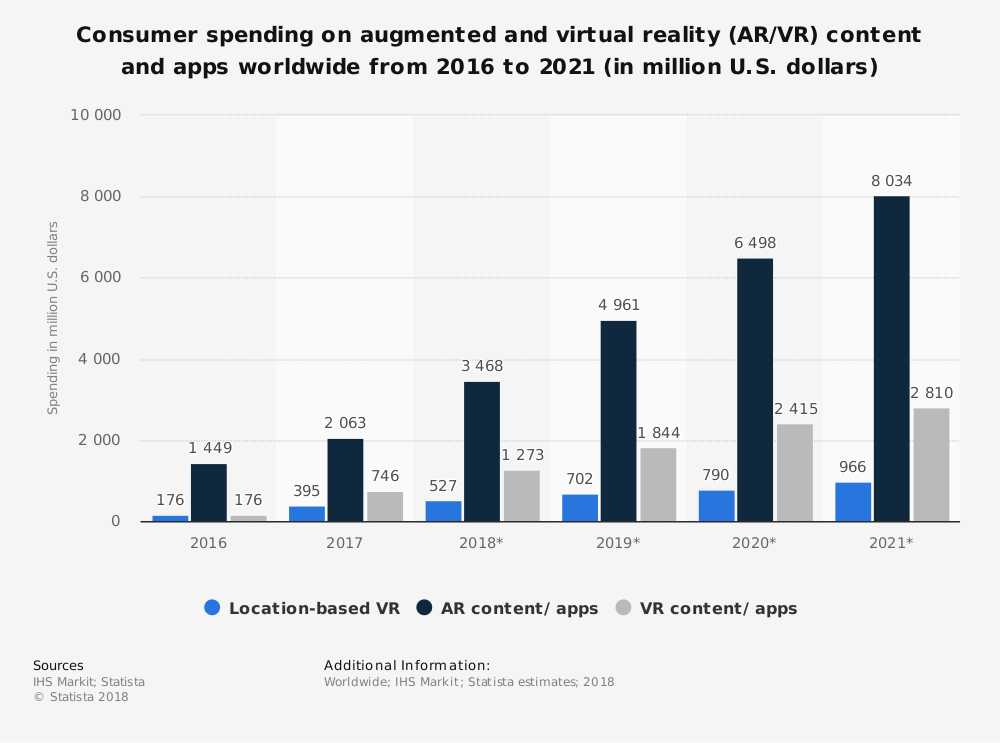
\includegraphics[height=210pt]{ar-vr-consumer-spending}
	\caption{\citep{ar-vr-chart}}
	\label{fig:ar-vr-consumer-spending}
\end{figure}
\chapter{\MakeUppercase{Augmenter Reality and Virtual Reality}}
Augmented reality and Virtual reality are technologies that offer a different view and experience to the physical world. They leverage similar kinds of technology and both aim to provide an enhanced and enriched experience to the user. Both technologies are a part of the general area of mixed reality \Cref{fig:reality-virtuality}. However they have different goals and are essentially different in terms of user experience.

\begin{figure}[H]
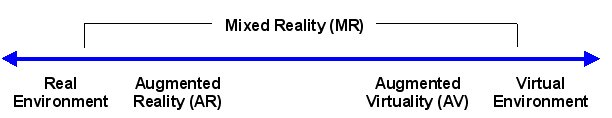
\includegraphics[width=\textwidth]{Virtuality_Continuum_2}
\caption{Reality-Virtuality Continuum (Paul Milgram et al. 2007)}
\label{fig:reality-virtuality}
\end{figure}

\section{Augmented Reality}%ref http://kjcomps.6te.net/upload/paper1%20.pdf
Augmented Reality can be described as the technology that bridges reality with virtual environments. Real life objects are transformed or replaced with virtual equivalents. Information can be added or removed to the real environment. Key aspects of AR(Augmented Reality) are the ability to run in real time, be interactive, three dimensional and combine real with virtual information\Cref{fig:ar-application}. AR is most commonly used with the sense of sight, but it can potentially be used with other senses such as hearing, touch, smell, taste, temperature etc. Augmented Reality can be considered as the next step in graphical user interfaces(GUI) evolution\citep{prototyping-ar}. Its current state is comparable to command line interfaces and 2d interfaces in the 1980's and 1990's. It is a vision of future computing and a field that is under research.
\begin{figure}[H]
	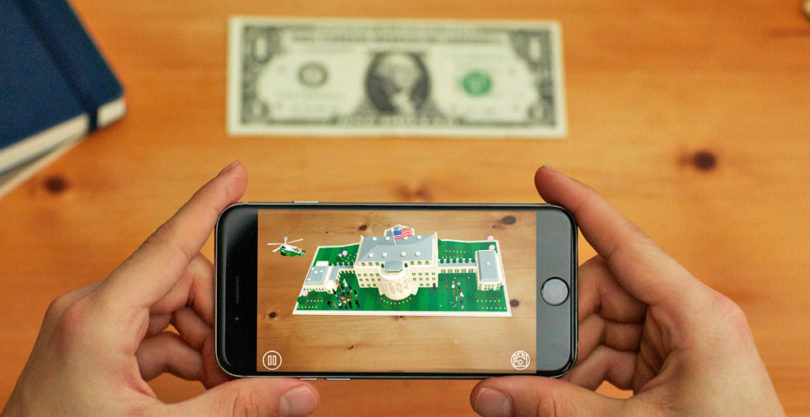
\includegraphics[width=\textwidth]{ar-application}
	\caption{Mobile Augmented Reality application\citep{ar-application-whitehouse}}
	\label{fig:ar-application}
\end{figure}
\par
Augmented Reality has higher technological requirements compared to VR which has lead to the slower maturity of AR. AR enabling technologies have been developed throughout the history of which the Optical see-through has become the most popular(Microsoft HoloLens, Google Glass, Intel's Vaunt). Optical see-through is achieved by using opaque displays on which virtual overlays can be rendered. The resolution of the real world is left intact as it passes through the screen. Benefits of this approach include power fail safety, which allows users to still see the real world even during a power outage, cheaper production costs of the used displays, no parallax effect that irritates the user's eyes. Disadvantages are the reduced visibility and brightness through the opaque lenses, limitation of the field-of-view, requirement of additional tracking sensors such as cameras, gyroscopes and accelerometers. Due to the lack of maturity of other AR enabling technologies only Optical see-through techniques will be considered throughout this work\citep{vrjournal}.
\subsection{AR for training and education}%ref https://files.eric.ed.gov/fulltext/ED510220.pdf
Augmented Reality provides new paths to conveying information. Learning experiences are more contextual by connecting and embedding information with the real world in real time. These approaches are already being utilised by Boeing. 
Mechanics in the company use AR goggles that aid repairs with embedded textual instructions, 
illustrate different steps of the repair and help users identify the required tools for a repair. 
Consequently training resources are reduced and transfer of information between workers is greatly 
improved\citep{horizon-report}.\par
Learning through doing is another approach in which AR shines. Mistakes and errors made during the learning
experience have no real consequences. This provides for more authentic learning experiences which cannot be
achieved easily or cost effectively otherwise\citep{augmented-reality}.
\subsection{AR Challenges}
% As most developing technologies AR has many challenges that need to be overcome or improved. The requirements of the AR framework
% are directly related to those challenges.
An AR framework has basic requirements to accomplish a combination of the real and virtual world.
The four main requirements are sensing, tracking, interaction and displaying\Cref{fig:ar-framework}. Sensing refers to
capturing environment events and recognising markers or other objects of interest. Tracking handles updating the
viewing direction and position of the user relative to the real world. Tracking is an important component
of AR as even a slight tracking error can cause misalignment between the virtual and real world objects\citep{ar-design}. 
Registration refers to how the digital information is being delivered to the user. The registration can be achieved
through different methods for different senses: videos, audio, haptic feedback, scent, etc.
\begin{figure}[H]
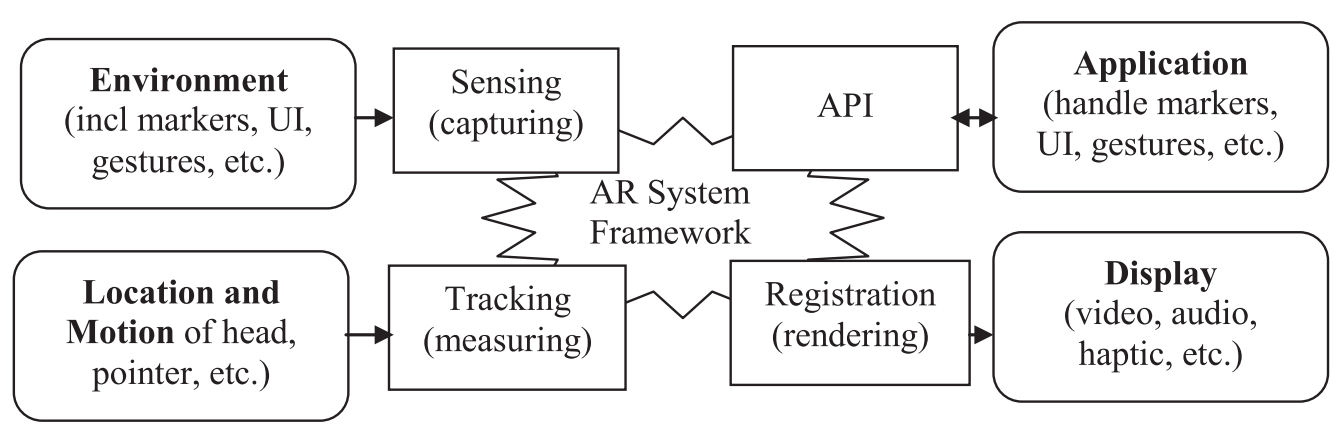
\includegraphics[width=\textwidth]{ar-framework}
\caption{Augmented Reality framework\citep{vrjournal}}
\label{fig:ar-framework}
\end{figure}
As most developing technologies AR has many challenges that need to be overcome before it can be widely adopted.
The challenges of AR arise from the framework requirements and they can be separated in five groups\Cref{fig:ar-challenges}.
\begin{figure}[H]
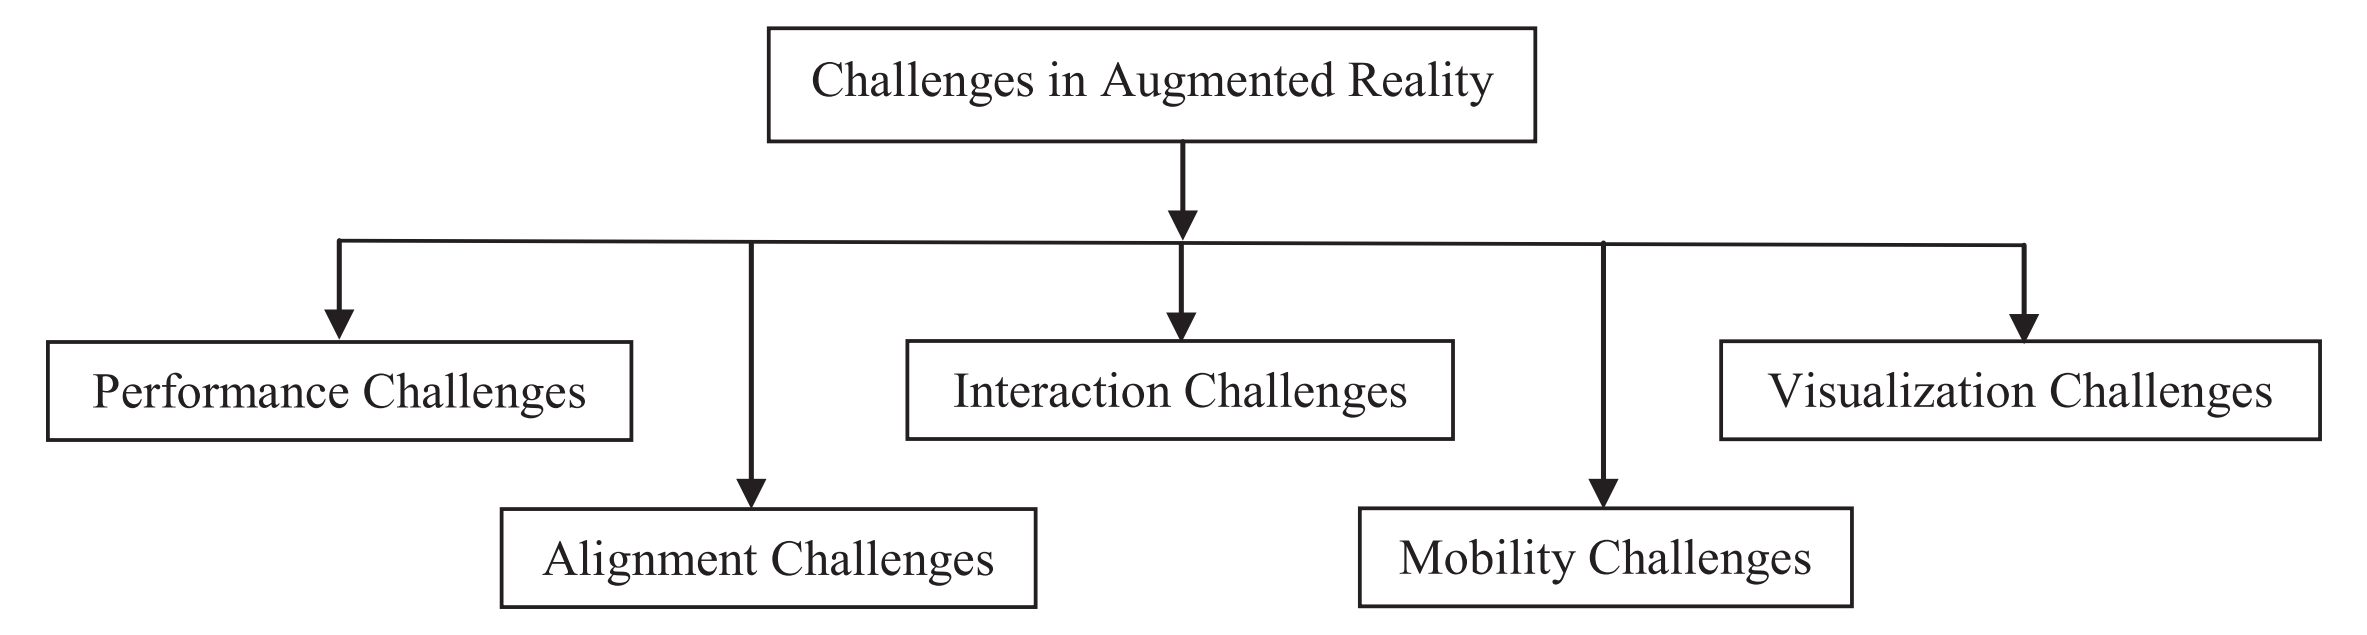
\includegraphics[width=\textwidth]{ar-challenges}
\caption{Augmented Reality challenges\citep{Acta-Graphica}}
\label{fig:ar-challenges}
\end{figure}
Performance challenges arise from the need of real time processing. AR tasks such as marker detection
and virtual object rendering are computationally intensive and this slows down performance.
Alignment challenges come from the complexity of tracking the users movement and registration of real
life objects. Any errors in those methods can cause misalignment between the rendered objects and
real view.\par
Interaction challenges are concerned with the interaction between users and virtual or real objects.
User interfaces need to be intuitive and unobstructive for the best experience. Mobility challenges refer
to the need of portability for AR systems.
\\
\section{Virtual Reality}
Virtual Reality in the broadest sense is the method or technology of substituting a physical environment with a virtually perceived environment. The Oxford dictionary gives a more detailed definition: 
''The computer-generated simulation of a three-dimensional image or environment that can be interacted with in a seemingly real or physical way by a person using special electronic equipment, such as a helmet with a screen inside or gloves fitted with sensors''.
This is typically achieved by using an HMD with integrated motion tracking and a built-in or external rendering unit.
The requirements of VR are same to those of AR with the exclusion of environment sensing\Cref{fig:ar-framework}. The virtual environment
is entirely digitally constructed, thus eliminating the need for sensing as all environmental events are native to the system. It is achieved with a Virtual Reality headset that has different views for each eye, accomplishing depth perception\Cref{fig:htc-vive-pro-headset}.
\begin{figure}[H]
	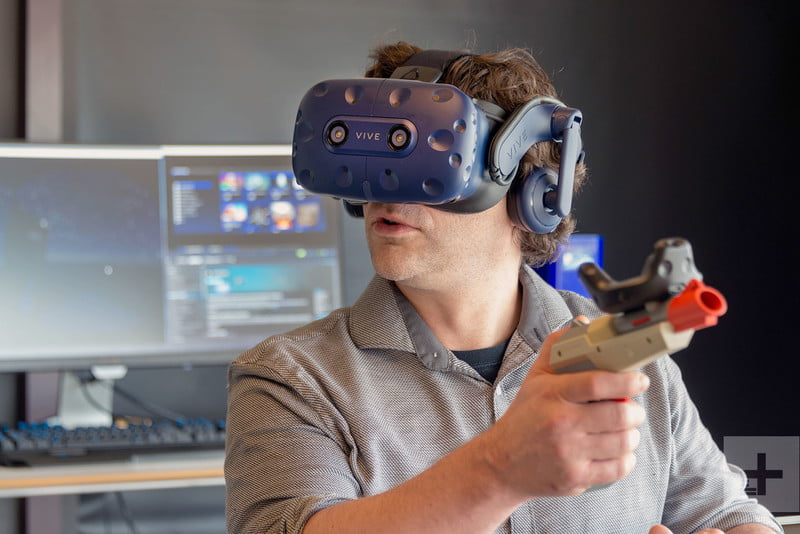
\includegraphics[width=\textwidth]{htc-vive-pro-headset}
	\caption{HTC VIVE Pro headset\citep{htc-vive-pro-review}}
	\label{fig:htc-vive-pro-headset}
\end{figure}
\par
Interaction with the environment isn't necessary for a VR experience, but it increases the possibilities and usability of a VR system.
Different approaches to user interaction offer various degrees of immersion and limitations. Motion tracked controllers, hand motion tracking gloves, pointer centered to the viewport, headset location tracking in 3D space and sekeletal motion tracking are common approaches.
\subsection{VR Challenges}
VR challenges can be categorized in the same way as AR challenges\Cref{fig:ar-challenges}.
Performance is a very important factor in keeping the VR experience immersive for a prolonged period of time.
High resolution picture rendering at a high freamerate in real-time is taxing even for the highest end of current GPUs. 
Lower framerate or lower resolution picture can cause dizziness, eye tiredeness and overall dissatisfaction. Alignment challenges arise from the difficulty of tracking in real-time.
Users' view, location or controllers can become misaligned with the virtual environment, breaking the immersion and interactability.
Interaction challenges come from the current hardware limitations on interacting. Tactile feedback, hand interaction and free movement in the 3D space are all possible individually, but combining them at the same time is not yet achievable.
\par %(Interrante et al., 2008; Mohler et al., 2010; Phillips et al., 2010).
Mobility challenges arise from the need of portability for VR platforms. Common solutions
rely on tethering to a machine that handles the rendering and power supply. However portable VR backpacks and headsets are starting to emerge\citep{hp-vrbackpack}.
Visualization can be difficult due to the complexity of the physical world. Keeping proportions, lighting, textures, view depth, field of vision and other visiual perception aspects can be challenging.
\subsection{VR for education and training}
VR has many prospects for use in education. Learning can be promoted by interacting with objects and the environment in a virtual world. 
Similarly self-paced exploration can improve the users' ability to understand a given topic.
%reference VR Collaborative learning
Learning through doing is even more prominent with VR than AR. Scenarios that are hard or impossible to create with traditional approaches can be executed in a virtual environment for the fraction of the cost.
Users that are physically apart can be in the same virtual environment.
Professors or specialists don't need to travel to remote locations to train people.
\section{Hybrid approaches}
\par
Hybrid approaches to VR and AR can be used to improve on some of the imposed drawbacks by the techologies. These approaches include using physical objects or combining different sensors.
Such a drawback for VR is the lack of tactile feedback or realistic hand interaction with the environment. This becomes a problem when training pilots as they get accustomed to the feel of the virtual environment and are unable to perform tasks as quickly in the real environment.
Feedback from the cockpit instruments is essential as well as the ability to use them with peripheral vision.
One solution to this problem has been developed by NLR with the use of a hybrid approach.
IR depth sensors and a camera feed are used to map the pilots hand in the virtual cockpit. Mockups of the flight instruments are 3D printed and are mapped to the virtual environment with tracking markers.
This allows for a much more natural feel of the flight instruments and offers better training results\citep{nlr-vr}.
\\
\chapter{\MakeUppercase{Project use case}}
Observis Oy is developing a product for situational awareness in different environments called ObSAS.
This product is a software system running on multiple devices with multiple purposes.
Low level software that communicates with various sensors and devices, Server software
that summarizes the data and handles automatic actions and the User software that allows users to interact
with all components of the system. The environment the software can be integrated 
into vary a lot and so does 
the complexity of the various applications associated with the product.
\par
The end use for the product is usually civil defence or shelter management.
High reliability and availability are crucial requirements for the final product as 
human lives can be put in danger by improper operation of the software or misuse by
the users. Training is becoming necessary to ensure proper use of the software and 
other components of the situational awareness system. So far traditional training 
approaches have been used. Power slides including pictures of the software, textual description of individual components and narration from the training personnel.
\par
\section{Current training approach}
Current training is done on customers premises in two parts - theoretical and practical. The theoretical part takes place in a classroom with teaching tools such as whiteboard and projector provided by the customer. A group of 20 people is trained during the theoretical part with the use of powerpoint slides containing screen captures of the software. Additionally the software enabled in simulation mode is displayed and used in front of the trainees. Devices such as latops, external hard drives, cameras are not allowed during the training to avoid redistribution of confidential information.
\par
The second part of the training involves practical use of the system. In the Sassi Project case it takes place inside a reconnaissance vehicle with a group of 3 to 4 people. Real life devices are used with the software. Test sources are used to trigger devices alarms and cable disconnecting is used to test failure states.
\par%switched to past perfect, not sure why, a bit inconsistent?
Feedback from the customer in the Sassi project has been positive, although there have been complaints from the trainees about the translation of the materials, but still overall positive feedback has been received. According to Jukka Härkönen(an employee from Observis who conducts the training) the trainees with better English language skills have managed to attain more knowledge from the training. Trainees who were familiar with a previous version of the software have had no problems adjusting to the differences in the new version of the product. Some trainees however have not been able to fully prepare for the use of the software and require further internal training conducted by the customer.
\section{Future goals}
Regardless of the good customer feedback there is room for improvement of the training. Streamlining of the training can reduce the time required to create training materials and the amount of staff needed to conduct the training. Another future goal of the training is to be able to experience more lifelike situations and more complex scenarios resulting in better preparedness for critical situations. Misunderstanding caused by a language barrier is something that should be avoided in future training.
\par
Innovation in every aspect of the product is welcomed from the customers. The market has been stagnant and competing companies have been refusing to innovate due to the various risks involved with doing so. Observis is willing to take those risks to set itself apart. A survey and analysis of Virtual reality technologies is of interest to the company.
\par
\section{Comparing VR and AR in the project context}
AR and VR differ not only in hardware but also in software development kits. It is rarely the case that an application written for one of the platforms can be seamlessly ported to the other. Therefore the two technologies need to be compared in regards to the current project. To keep the scope of this thesis narrow a single technology will be used to implement a training application.
\par
AR hardware such as goggles, glasses and headsets are generally very portable and self-contained. This makes it easy to transport the required hardware during training or installation tirps. The initial setup of the training environment could be more tedious with AR. If real life devices need to be tracked, markers have to be placed and calibrated. Immersion may be sacrificed due to the narrow field of view\citep{hololens-specs}, smaller color space, low luminosity and lower computing power. Another downside is the inability to emulate real life scenarios such as being inside a moving vehicle or simulating an environment that is completely different from the one the user is in. For example it is impossible to simulate night missions if the user is in a brightly lit room. For these reasons AR is restricted by the environment it is being experienced in.
\par
The easability of use of AR headsets is one important benefit. While VR headsets require a tether cable, external computer and even base stations in some cases, AR headsets can be used as they are, independently. 3D modelling isn't as big of a requirement compared to VR as it is enough to create models only of the objects the user interacts with, not the full environment the user is in. This can reduce development time significantly.
\par
VR shines in implementing a completely independant environment. The only limit to what can be recreated is imposed by the hardware performance and development time and skills. VR allows for spectating and recording users' interaction with the environment. This can be used to analyze their experience and improve the software further. Giving suggestions and guiding during the training is also possible. A multi-user environment is also possible and trainees and teachers can be in the same environment even if they're physically far apart.
\par
Price difference is very small between VR and AR if the most advanced frameworks are being considered. An AR headset with the development pack such as Microsoft HoloLens is priced at 3000\$\citep{hololens-price}. And a VR headset such as HTC Vive Pro is priced at 1500\euro\citep{htc-vive-pro} with VR capable laptops priced starting from 1500\euro. Similarly prices of development kit licenses are not far apart either. This makes the decision between the two based entirely on the features they provide, driven by the requirements of the use case they're aimed for.
\par
\section{Defining the application specifications and requirements}
The primary goal of the training application is to provide a better view on the future prospects of using mixed reality for training. A secondary goal is to offer a training platform for better understanding of the ObSAS software to trainees. Furthermore finding other suitable AR/VR use cases for the current Observis projects can also be a positive by-product of the research.
\par

\section{Selection of mixed reality framework}
\par
\chapter{\MakeUppercase{Project implementation}}
\section{Researching mixed reality implementation}
\section{Risks and challenges to the mixed reality approach}
\section{Implementing basic scene with objects}
\section{Tracking and interacting with the virtual environment}
\section{Creating a context for training}

\par
\chapter{\MakeUppercase{Analyzing the mixed reality training application}}

\section{Future possibilities for development and improvement}


\newpage

\nocite{*}
\bibliography{references}

\end{document}
